\documentclass[paper=a4,fontsize=11pt,twocolumn,pagesize,bibtotoc]{scrartcl}

\usepackage[utf8]{inputenc} 
\usepackage[T1]{fontenc}
\usepackage[english]{babel}

\usepackage[osf]{mathpazo} 
\usepackage{microtype}
\usepackage{tikz}
\usetikzlibrary{automata}
\usepackage{amsthm, amssymb, amsmath}
\usepackage{graphicx}
\usepackage{color}
\usepackage{hyperref}

\usepackage{circuitikz}
\usepackage{pgfplots}

\parindent0pt


\title{cmidid}
\subtitle{usage and configuration of the module}
\author{Jannik Theiß}

\begin{document}
\maketitle

The purpose of our module is to enable musicians who also like to tinker or tinkeres who also like to make music to build their own custom MIDI input device. A MIDI input devices consists of multiple triggers, which form the intrument. A trigger can for example be a key of a convetional keyboard or a drumhead of an electronic drumkit. The musician then interacts with the triggers to initiate the production of a MIDI event which is then used to produce a sound. Typically every trigger is assigned to a certain note which determines the pitch of the sound. More advanced triggers however can produce MIDI events with different velocities depending on how hard the musician hits the trigger.

To build a custom MIDI device the triggers have to be constructed and connected to the GPIO ports. Our module can then be configured to be controlled by these triggers. It supports normal keyboard keys and similar constructions with velocity measurement. It is also possible to construct triggers that look different than keyboard keys but follow the same logic. The module implements the the logic for the keys to and produces the MIDI events which can then be routed via ALSA.

\section{construction of a key}
To be able to produce MIDI events with different velocities, we measure how long it takes for the key from the inital position to be fully pressed down when it is hit by the musician. Our experiments have shown that this time is a reasonable approximation to the force that was used to hit the key.

To enable the time measurement we use two momentary switches per key. The first switch is closed (or opened, depending on the construction) when the key starts to move. The second one is closed (opened) when the key reaches the bottom position. The physical construction of a key could look like this: the key is pivot-mounted on its back side and held up with a spring on its front. The first switch is above the key and will be closed as long as the key isn't moved. The spring holds the key in this initial position. As soon as the musician hits the key, the first switch will be opened. The second key is positioned under the key and will be closed when the key is fully pressed down.

As the Raspberry Pi has 17 GPIO ports and we need two GPIO ports per key, it can be used to construct devices with up to 8 keys.

\subsection{key logic}
The key logic determines the situations in which a trigger should cause a MIDI event to be produced. There are two different types of MIDI events which are important in this situation: note-on and note-off events. Note-on events will cause a sound to start and note-off events for the same note will cause the sound to stop. If there are multiple note-on events for the same note, the same number of note-off events has to be produced to stop the sound.

The state-machine in figure \ref{fig:state} describes the key logic in our module. There are three states: \texttt{inactive}, \texttt{touched} and \texttt{pressed}. As long as a key is in its inital position, it should stay in the \texttt{inactive} state. The \texttt{touched} state describes the situation that the key started to move but wasn't fully pressed down yet. As soon as the key is fully pressed down, it will transition to the \texttt{pressed} state until it is released completely and goes back to the \texttt{inactive} state.

The actions of the two swichtes $b_1$ and $b_2$ will cause the transitions between the states. If $b_1$ is activated in the \texttt{inactive} state, the key will transition to the \texttt{touched} state and a counter starts counting the time. If next $b_2$ is activated, the key was fully pressed down. It will go to the \texttt{pressed} state and the elapsed time will be used to compute the velocity for a new note-on event, which will then be produced. A situation which can't be hanled perfectly by our construction occurs, when a key is pressed down a second time before releasing it completely. As $b_1$ won't be activated in the moment the key was hit, we can't measure the time of the key movement. We therefore decided to produce a note-on event with the same velocity as the event before whenever $b_2$ is activated in the \texttt{pressed} state. We also have to produce a note-off event for the note-on event that was produced by the first activation of $b_2$. On releasing the key, $b_1$ should be deactivated and the key goes back to the \texttt{inactive} state. This is equally true for all states. We also produce a note-off event in this situation, which will stop a previously started sound. This is not alway neccecary (for example in the \texttt{touched} state) but provides some robustness against failures which could for example occur due to imperfect debouncing of the switches. Thereby the musician can be sure, that the sound stops when the key is released.


	\begin{figure}
		\centering
		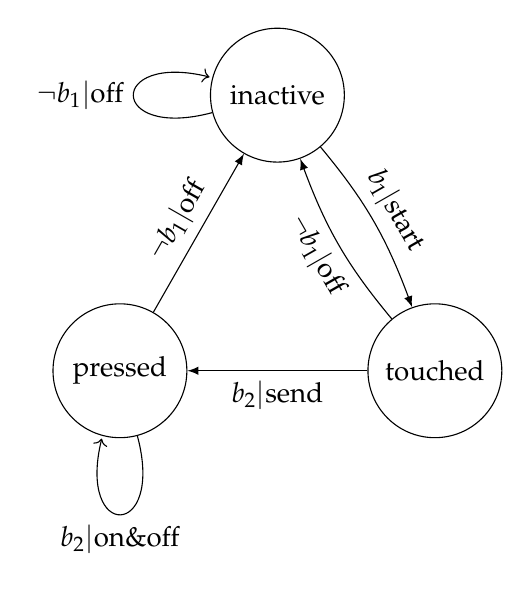
\begin{tikzpicture}[node distance=3cm,bend angle=10]
	        \node[state,minimum size=1.7cm] at (0,0)   (act) {inactive};
	        \node[state,minimum size=1.7cm] at (2,-3.5)  (touch) {touched};
	        \node[state,minimum size=1.7cm] at (-2,-3.5)  (press) {pressed};
		
			\path[-latex] (act) edge[bend left] node[sloped,above] {$b_1|$start} (touch)
					(touch) edge node[sloped,below] {$b_2|$send} (press)
							edge[bend left] node[sloped,below] {$\neg b_1|$off} (act)
					(press) edge node[sloped,above] {$\neg b_1|$off} (act);
		\path[-latex] (press) edge [loop below] node {$b_2|$on\&off} ();
		\path[-latex] (act) edge [loop left] node {$\neg b_1|$off} ();
		\end{tikzpicture}
		\caption{key logic}
		\label{fig:state}
	\end{figure}

\subsection{wiring}
The switches $b_1$ and $b_2$ can be connected to the GPIO ports of the Raspberry Pi with the pull-up circuit shown in figure \ref{fig:circuit}. Alternatively a pull-down circuit or a circuit suited to other than normal momentary switches can be used. When the switch is open the circuit in figure \ref{fig:circuit} draws no power, as the port is configured as input an thus there is no current flow. Because no current flows through the resistor, there is no voltage drop across it and therefore the GPIO port is pulled to $3.3V$ or logical $1$. When the switch is closed the port pulled down to ground level or logical $0$. In that case the $3.3V$ is connected to ground via the resistor and a current of $3.3V / 33k\Omega = 0.1mA$ drawn. Resistors with other values can also be used, but as the resistor acts as a limiter for the current, care has to be taken that the pins of the chip are not overloaded.

\begin{figure}
\begin{circuitikz}
	\centering
			
			\draw (0,0) to[short] (2,0) to[cspst] (2,2) to[short,-*] (1,2); 
			\node[right] at (2.2,1) {switch};
			\draw (0,0) node[ground] {};
			\draw (0,-0.5) node[below] {ground};
			\draw (0,4) node[left]{3.3V} to[short] (1,4) to[resistor=33\,$k\Omega$] (1,2) to[short] (0,2) node[left]{GPIO}; 
		\end{circuitikz}
		\caption{pull-up circuit}
		\label{fig:circuit}
\end{figure}

\subsection{possible extensions}
There are several possible extensions which are currently not implemented by our module. Adding support for a sustain pedal would be indispensable, if the MIDI device should be used as a traditional piano. However for playing sythesizer sounds, a sustain pedal is non-essential. More advanced features could include support for pitch and mod wheels, aftertouch and the posibility to split the keyboard in different zones which can send MIDI events on different and possibly multiple channels simultaneously.
It would also be nice to support different types of triggers such as electronic drumhead. However this would require to rework central party of the module because of the fundamentally different logic behind these. In addition the configuration of the module would become more complex as it would require a more detailled definition on how the triggers are built.

\section{module configuration}
Our module provides considerable configuration possibilities via module parameters and \texttt{ioctl} to support different wirings and allow some fine-tuning. Some of the configuration possibilities are accessible through both module parameters and \texttt{ioctl}. This allows for flexible experimenting with these parameters without the need to call the \texttt{ioctl} command after every time the module is loaded.

\subsection{module parameters}
Module parameters are used for static configuration that is unlikely to change during the usage of the module such as parameters specific to a certain construction of a trigger. These parameters must be provided when the module is loaded. They are declared with the \texttt{module\_param} or \texttt{module\_param\_array} macro.

\subsubsection{GPIO mapping}
The \texttt{gpio\_mapping} parameter array is used to specifiy to which GPIO ports the switches of the keys are connected. The array has to be filled with three integers per key. If the number of provied integers is not dividable by three, the module loading will fail.

The first two of each three numbers are the GPIO numbers for the first and second switch. The third number is the midi note (in halftones, $a'$ is 69) which will be associated with the key. It is currently not checked wether two keys are instanciated with the same note, but this could lead to unwanted effects.

As the user of the module has the choice which notes are used, it is possible for devices with a small number of keys to use non-adjacent notes. A device with four keys could for example realize a simple chord or some specific notes for a MIDI drumkit.

\subsubsection{polarity of the buttons}
The \texttt{start\_button\_active\_high} and \texttt{end\_button\_active\_high} parameters are booleans that have to be set according to the electrical and logical polarity of the switches $b_1$ and $b_2$. We assume that all triggers are constructed the same way, so these parameters affect all of them. If the start button produces a rising edge (a transition from ground to $3.3V$) when it is activated, \texttt{start\_button\_active\_high} has to be set to true. Activated means (defined in the state-machine in figure \ref{fig:state}) in the case of $b_1$ that the corresponding key started its motion, whereas deactivated means that the key was released. This behavior depends on both the electrical connection of the switch (pull-up or pull-down circuit) and the physical construction of a key (will the button be closed or opened when it is activated).

\subsubsection{debouncing time}
Because we want the time measurement to be as precise as possible, we decided not to debounce the switches in hardware, which would delay the signal. Therefore the debouncing has to be realized in software. The \texttt{jitter\_res\_time} parameter specifies a time span during which subsequent signals from a switch are ignored. Shorter times result in more faulty recognized edges, longer times in ignoring legitimate edges. A practical value depends highly on the construction of a key. We made this constant therefore configurable. For our testing setup values between $500\mu s$ and $10ms$ resulted in acceptable behaviors.

\subsubsection{stroke times}
These values affect the mapping from measured stroke times to MIDI velocity values, which range from 0 to 127. \texttt{stroke\_time\_min} and \texttt{stroke\_time\_max} minimal and maximal times used for the velocity curve as explained in section \ref{vel}. The times are specified in $2^{10}$ nanoseconds. \texttt{stroke\_time\_min} and shorter times result in a velocity value of 127, \texttt{stroke\_time\_max} and longer times result in a value of 0. These values can also be dynamically controlled with \texttt{ioctl} (see calibration in section \ref{calib}). \texttt{ioctl} can then output the new values to use them for static configuration with these module parameters. In this way, the values from a calibration can be loaded upon module loading.

\subsubsection{midi channel}
The \texttt{midi\_channel} parameter is simply the midi channel which is used for the produced MIDI events. As a possible improvement this could be configured via \texttt{ioctl} rather than a module parameter, which would allow to switch the channel while playing.

\subsection{ioctl}
\texttt{ioctl} allows to control a module which is already loaded. It can be used for dynamic configuration of parameters that are not specific to the setup and which the musician might want to change while playing the intrument.

The headerfile \texttt{cmidid\_ioctl.h} includes the possible ioctl commands which are described in the following section.

\subsubsection{stroke time calibration}
\label{calib}
When \texttt{ioctl} is called with \texttt{CMIDID\_CALIBRATE\_MIN\_TIME} or \texttt{CMIDID\_CALIBRATE\_MAX\_TIME} the measured time of the last key stroke is used for the respective value. This enables the dynamic calibration of the force needed to produce notes with minimal and maximal velocity. The value returned by \texttt{ioctl} can later be used with the module parameters to use the same values again after reloading the module.

\subsubsection{velocity curves}
\label{vel}
As the minnimal and maximal times define the values mapped to velocity 127 and 0, the velocity curve is responsible for mapping all values in between. There are four different velocity curves implemented in our module whih can be selected by passing \texttt{CMIDID\_VEL\_CURVE\_LINEAR}, \texttt{CMIDID\_VEL\_CURVE\_CONCAVE}, \texttt{CMIDID\_VEL\_CURVE\_CONVEX} or \texttt{CMIDID\_VEL\_CURVE\_SATURATED} to \texttt{ioctl}. The different curves can be seen in figure \ref{fig:vel}. By selecting the appropriate curve, the musician can choose which area is more dominant in the mapping, which enables a more precise play in that area. For example the concave curve has a wider area of time differences mapped to low velocities and it is therefore easier to play precise with low velocities.

\begin{figure}
	\centering
	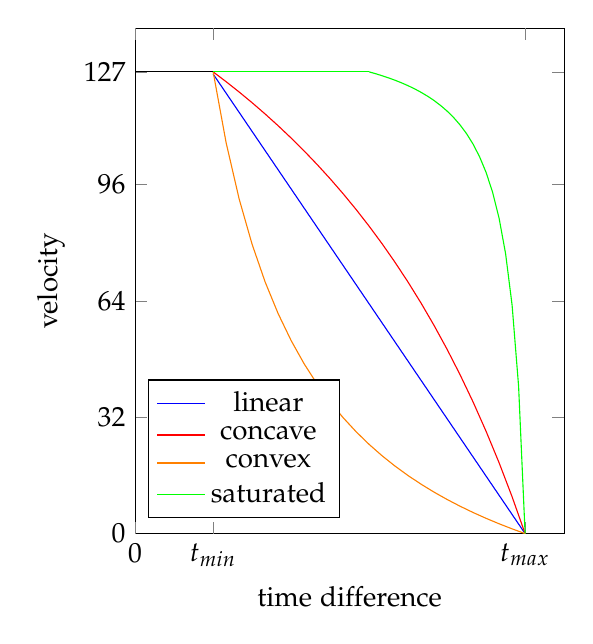
\begin{tikzpicture}
		\begin{axis}[width=200pt,xtick=\empty,extra x ticks={0,20,100},extra x tick labels={$0$,$t_{min}$,$t_{max}$},ytick={0,32,64,96,127},height=8cm,ymin=0,ymax=139,xmin=0,xmax=110,ylabel={velocity},xlabel={time difference},log basis y={2},legend pos=south west]
			\addplot[draw=blue,domain=20:100] {-1.58*x+158};
			\addlegendentry{linear};
			\addplot[draw=red,domain=20:100] {20560.6/(x - 180.63) + 255};
			\addlegendentry{concave};
			\addplot[draw=orange,domain=20:100] {4207.87/(x + 5.19685) - 40};
			\addlegendentry{convex};
			\addplot[draw=green,domain=60:100] {573.228/(x - 104.094) + 140};
			\addlegendentry{saturated};
			\addplot[draw=black,domain=0:20] {127};
			\addplot[draw=green,domain=20:60] {127};
		\end{axis}
	\end{tikzpicture}
	\caption{velocity curves}
		\label{fig:vel}
\end{figure}

\subsubsection{transpose}
By sending \texttt{CMIDID\_TRANSPOSE} with a value in halftones, all produced MIDI events will shift their note by this value. \texttt{ioctl} returns then the current transpose plus 128. So by sending \texttt{CMIDID\_TRANSPOSE} with 0, the current transpose can be read from the module.

A minor problem that is not solved in out module is that started notes might not stop, if the transpose is changed inbetween, because there is no key assigned to that note anymore.

\section{conclusion}
Our module provides all the functionality that is needed to build a custom MIDI input device with the Raspberry Pi. All parameters that are needed to support different key constructions are accessible via module parameters. In addition we provide some options for fine tuning via \texttt{ioctl}.
	
	
	
\end{document}